\documentclass[11pt]{article}
\usepackage[margin=1in]{geometry}          
\usepackage{amsthm}
\usepackage{amsmath}
\usepackage{amssymb}
\usepackage{csquotes}
\usepackage{setspace}\onehalfspacing
\usepackage[loose,nice]{units} %replace "nice" by "ugly" for units in upright fractions
\usepackage{graphicx}
% \graphicspath{ {/Users/eghuang/math104/images/} }
\usepackage{listings}
\usepackage{color}

\definecolor{dkgreen}{rgb}{0,0.6,0}
\definecolor{gray}{rgb}{0.5,0.5,0.5}
\definecolor{mauve}{rgb}{0.58,0,0.82}

\lstset{frame=tb,
  language=R,
  aboveskip=3mm,
  belowskip=3mm,
  showstringspaces=false,
  columns=flexible,
  basicstyle={\small\ttfamily},
  numbers=none,
  numberstyle=\tiny\color{gray},
  keywordstyle=\color{blue},
  commentstyle=\color{dkgreen},
  stringstyle=\color{mauve},
  breaklines=true,
  breakatwhitespace=true,
  tabsize=3
}

\title{
	Analysis on Seshat dataset \\
	\bigskip
	}
\author{Jaeweon Shin \space Brendan Tracey \space Hajime Shimao \\ Michael Price \space Tim Kohler \space David Wolpert}
\date{Summer 2018} 
 
 \newcommand{\R}{\mathbb{R}}
 \newcommand{\Q}{\mathbb{Q}}
 \newcommand{\Z}{\mathbb{Z}}
 \newcommand{\N}{\mathbb{N}}
 \newcommand{\B}{\mathbb{B}}
 \newcommand{\Prob}{\mathbb{P}}
 \newcommand{\E}{\mathbb{E}}
 \newcommand{\code}[1]{\texttt{#1}}
 \let\oldemptyset\emptyset
 \let\emptyset\varnothing
 
 \setlength{\parindent}{0pt} % no indent
\begin{document}
	\maketitle
	
	\begin{abstract}
		In 2017, a group of researchers (Turchin et al 2017) published a large database of historical records called Seshat. Using this dataset, the same researchers concluded that there is a major axis of social complexity, which  represents how complex a society is at a given time period. By expanding on this analysis, we show that there are, in fact, two clusters within the major axis that displays different characteristics. Furthermore, we show that these two clusters could imply that all societies could be classified into largely two stages based on the relative complexities of their societies. 
	\end{abstract}
	
\section{Background}
A majority of the historical research uses qualitative text-based analysis to infer the past. However, this approach is inherently limited in gaining a systematic overview of history. To resolve this, using quantitative approach to history was suggested by multiple scholars. Unfortunately, we did not have the data to utilize such quantitative tools, at least until last year. In 2017, a group of researchers (Turchin et al 2017) rendered efforts from multiple disciplines to gather historical records and published a large database of the past. \\
This dataset, called Seshat, is consisted of 414 societies where each society is described by 51 social variables, including but not limited to the size of the population, territorial size, and existence of written records. Each society is drawn from pre-defined 30 National Geographic Areas (NGA), where each National Geographic Area is a geographic region that contains one society at a time. Publishers of the dataset carefully crafted 30 National Geographic Areas that are relatively evenly distributed throughout the globe because uniform sampling in geographical sense is necessary to assess the development of independently developed societies around the globe. \\
In a paper published along with the dataset, Turchin aggregated the 51 social variables into 9 Complexity Characteristics variables to evaluate the complexity of a society. These 9 Complexity Characteristics variables are as follows: Information system, monetary system, government, hierarchy, texts, population size, territory size, capital population, and infrastructure. Then he ran Principal Component Analysis on this dataset with 9 features and found that there is one Principal Component that explains most of the variance of the data. Furthermore, he demonstrated that this Principal Component is positively correlated with time. Combining these findings, Turchin concluded that this main Principal Component represents the axis of social complexity. In other words, this Principal Component describes the system-level trajectory of how complex societies are over time. 

\begin{center}
	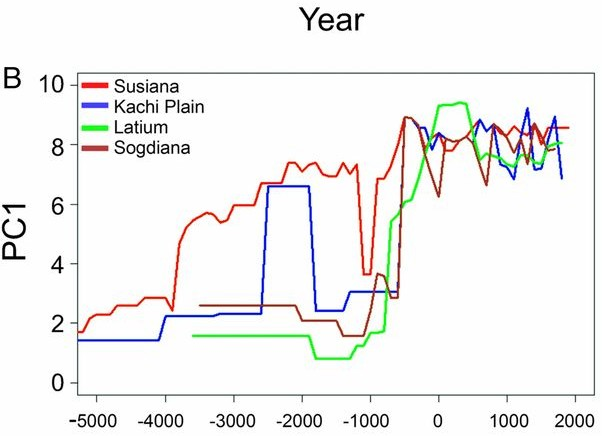
\includegraphics[scale=0.30]{time_pc.jpg}
	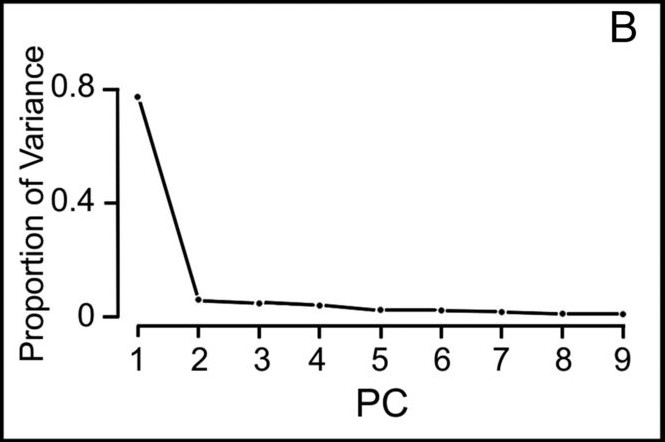
\includegraphics[scale=0.25]{pc_variance.jpg}
\end{center}

\section{Expanding on Principal Component Analysis}

As Turchin has previously shown, there is a single Principal Component that potentially represents the social complexity. A natural question to ask is, what are some dynamics that we observe along this principal component? In order to answer this question, we projected the data in 9-dimensional space on the 1-dimensional Principal Component axis. The resulting histogram of that projection is, as shown below, a bimodal curve. 

\begin{center}
	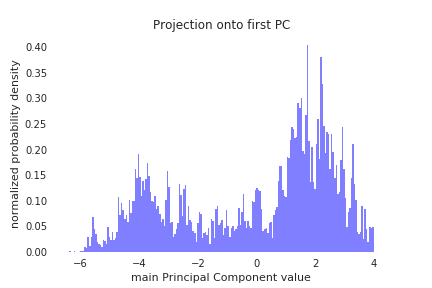
\includegraphics[scale=0.55]{first_PC.png}
\end{center}

The fact that the projection is bimodal shape could have multiple implications. First of all, the dynamics of social evolution is more complex than the single axis of social complexity Turchin suggested. Recall one of Turchin's findings that the main Principal Component is positively correlated with time. Given the positive correlation with time, we hypothesized that this bimodality suggests that all societies can be grouped into two different stages of social complexity. Furthermore, these two different stages of social complexity might be classified by non-major principal components that Turchin did not consider thoroughly. 

\section{Exploring various characteristics of bimodality}
Given bimodal curve we observed, we set out to explore various characteristics of the bimodality. In particular, to evaluate the potential effect of non-major principal components, we visualized a scatter plot of the most dominant and the second most dominant principal components as below, where dominance is defined by how much proportion of variance of the data the component accounts for. 

\begin{center}
	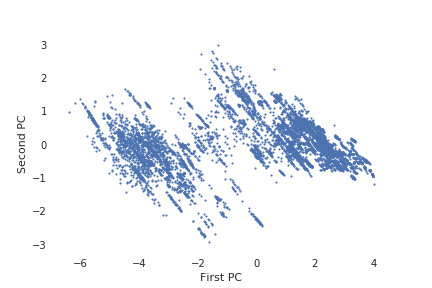
\includegraphics[scale=0.55]{two_PC.png}
\end{center}

As can be seen above, there are two large clusters of data points. To examine what these clusters represent, we used Gaussian mixture model on the dataset by fitting two Gaussians, where the choice of using two Gaussians was made because of the observed bimodal curve. Then we colored each data point with either red or blue, depending on to which of the two Gaussians the data point has a higher probability of belonging. As can be seen in the plot below, it turns out that the two Gaussians rather accurately distinguishes the two clusters. 

\begin{center}
	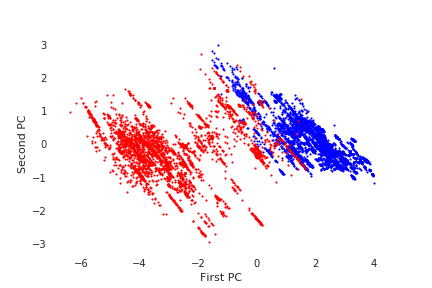
\includegraphics[scale=0.55]{two_pc.png}
\end{center}

To ensure that these two Gaussians are not closely aligned with each other, and that they are distinctive, we computed the angle between the eigenvectors that correspond to the largest eigenvalues for the covariance matrices for Gaussians. The computed angle was 33.56 degrees, which is large enough to conclude that these two Gaussians are not the same. \\

Another approach we attempted to assess bimodality was through plotting the overall trajectory of societies in each NGA. To do so, we first performed linear interpolation for all missing time periods within each NGA because some NGA had missing times between different societies. Then we plotted the trajectory of each NGA over time with respect to its main (dominant) principal component values with each NGA colored differently:

\begin{center}
	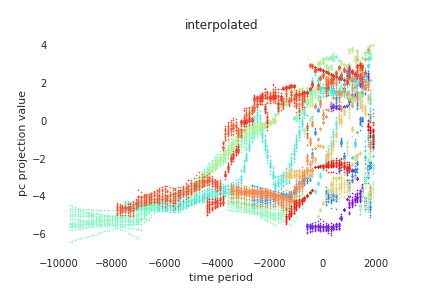
\includegraphics[scale=0.75]{interpolated_scatter.png}
\end{center}

One can observe from the above plot the two clusters nearby principal component value of -4 and 2, as we have noted on the bimodal curve. An interesting attribute of these trajectories is that most NGAs followed a constant path within each cluster in that the principal component value does not change much, and at some point, made a rapid leap from the bottom cluster to the top cluster. We suspect that this rapid jumps between the two clusters occur because of some attributes that distinguish the two clusters. For instance, it could be that once a society in the bottom cluster invents writing system, the society makes a jump and puts itself on the upper cluster. In another hypothetical situation, it is possible that a society in the bottom cluster gains momentum as it evolves and experiences exploding population, which pushes it to be in the upper cluster. 

\section{Resolving the undersampling bias}

One thing we'd like to ensure is that the bimodality is not an artifact of some biases. For this project, we mainly considered the undersampling bias that was conceivable in the context of archeology. By the nature of their field, archeologists are more inclined to research pre-historic societies. Furthermore, modern records are naturally more easily accessible and can be found in abundance. Thus, one hypothetical scenario is that the bimodal curve, in particular the trough region, is caused by nonuniform distribution of sampling. To address such undersampling bias, we performed two experiments: 1) linearly interpolating the missing time periods within each NGA and 2) weight different time periods based on their sparsity. The histograms for the result of the aforementioned methods are as follows:

\begin{center}
	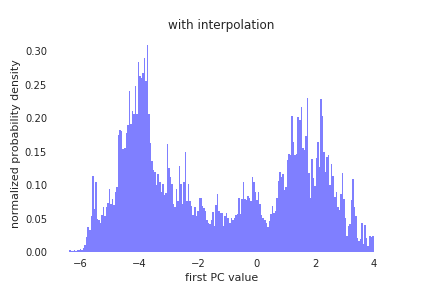
\includegraphics[scale=0.50]{interpolation.png}
	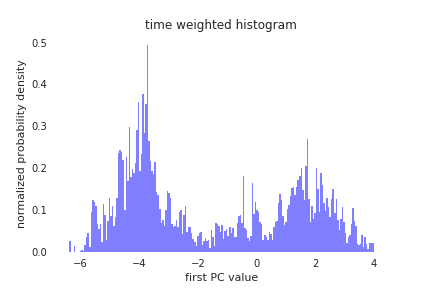
\includegraphics[scale=0.50]{time_weighted.png}
\end{center}

One can easily check that the bimodality survives both of these tests, which implies that the bimodality is at least not an artifact of undersampling bias. 

\section{Discussion}

The major finding of this project is the existence of two clusters along the first principal component, which accounts for the largest proportion of variance in the Seshat dataset. We have so far explored various characteristics of these two clusters, and addressed the issue of undersampling biases. To further this work, one could explore the defining features of the two clusters, namely what complexity characteristics variables distinguish the two clusters.\\
 In addition, one could explore the dynamics of societies over time with respect to each cluster. More specifically, we suspect that society displays different behaviors based on which of the two clusters it belongs. For instance, one possible scenario is that a society follows a negative-sloped trajectory within each cluster and follow a rapid positive-sloped trajectory at the boundary between the two clusters. Should each cluster display different behaviors, it could be an another indication of the distinctive nature of the two clusters.  

\section{Acknowledgements}

This project is a collaborative project with David Wolpert, Brendan Tracey, Hajime Shimao, Michael Price, and Tim Kohler with equal contribution from all of the collaborators. First, I would like to thank David for his advice and support throughout the project. We would not have had what we currently have had it not been for David to provide brilliant ideas and advices throughout the summer. I would also like to thank Mike, Hajime, and Brendan for all the advices they have offered me during the summer. Lastly, I would like to thank Tim for providing me with background anthropological knowledge to understand the results more clearly in the context of anthopology. 

\section{References}
Turchin, Peter, et al. “Quantitative Historical Analysis Uncovers a Single Dimension of Complexity That Structures Global Variation in Human Social Organization.” PNAS, National Academy of Sciences, 9 Jan. 2018.In-text Citation\\

Turchin, and Peter. “Fitting Dynamic Regression Models to Seshat Data.” Berkeley Planning Journal, 30 June 2018.


\end{document}